\chapter{Reconhecimento de Expressões Faciais}

\section{Introdução}
Segundo \citeonline{FernandoGil} "a expressão facial é uma forma de comunicação não-verbal que permite a partilha de
sentimentos e emoções, numa linguagem subentendida entre seres humanos". Desde o início das pesquisas na computação busca-se cada vez mais dotar o computador de um comprtamento inteligente. Sequindo esse caminho, o reconhecimento facial surgiu,  para trazer soluções no campo da Interface Home- Computador, como um desafio esperado, porém desafiador. Principalmente no reconheciemnto de expressões faciais, já que se trata de um julgamento ambíguo até mesmo para os seres humanos, pois a mesma expressão pode variar de indivíduo para indivíduo \cite{FernandoGil} \cite{Elizabeth}.

\section{Fasesdo Reconhecimeto}
O reconhecimento facial se divide em três etapas básicas \cite{Elizabeth}:
\begin{itemize}
\item Detectar a face na cena: Inicialmente é apresentada uma imagem contendo a face que deve ser rceonhecida. Nesta primeira etapa, deve ser realizada a detecção da zona da face, e devem ser extraídos os outros artefatos que não compõem o rosto \cite{FernandoGil}.
Na figura abaixo é ilustrado o resultado final desta primeira etapa.
\begin{center}
	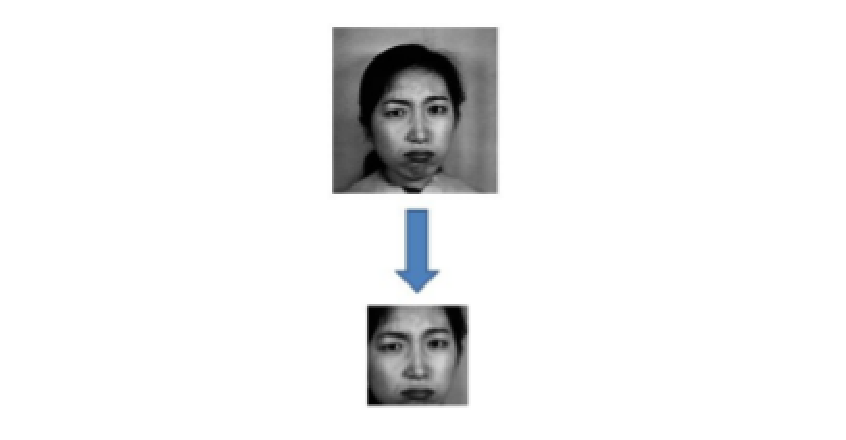
\includegraphics[scale=1.00]{graficos/rosto}
	\captionof{figure}{Detecção da face}
	\cite{Elizabeth}
\end{center}
\item Extrair as principais características: Nesta etapa são extraídas as características que são relevantes à classificação da expressão. Normalmente é dada maior ênfase as sobrancelhas, nariz, olhos e boca.
A figura abaixo mostra a seleção de pontos mais relevantes para a classificação da expressão
\begin{center}
	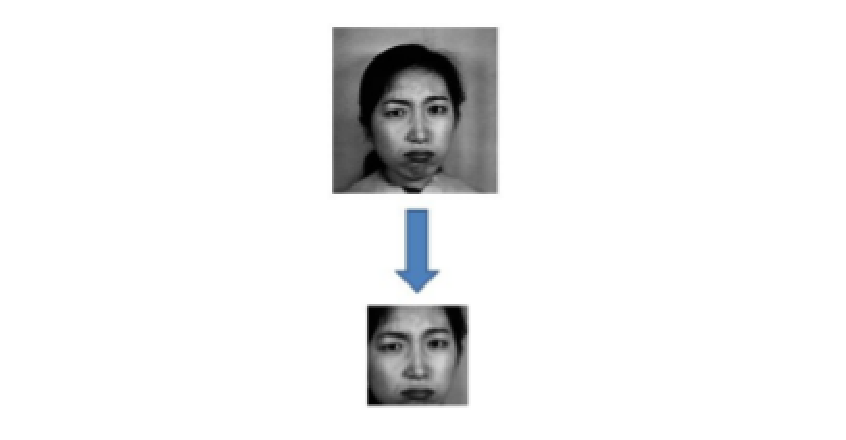
\includegraphics[scale=1.00]{graficos/rosto}
	\captionof{figure}{Pontos mais relevantes na face}
	\cite{Guo}
\end{center}
\item Classificar a imagem em uma detreminada expressão: 
\end{itemize} 


\section{Métodos Utilizados}

\section{A Programação Linear e o Reconhecimento de Expressões Faciais}
